%\chapter{Proposed - Potentiation in a simplified model}
%\chapter{Proposed - Bitstrings and potentiation landscapes: Insights from a simplified model}
%\chapter{Proposed - Potentiation landscapes and epistasis: Insights from a simplified model}
\chapter{Proposed - Epistasis and potentiation landscapes: Insights from a simplified model}
\label{chap:simplified_model}
\noindent
Authors: Austin Ferguson and Charles Ofria

\noindent
Status: Proposal. A small sample of preliminary data has been collected to help estimate time requirements and to verify that we do see meaningful levels of potentiation in NK landscapes. 

% \noindent
% Note: This chapter is proposed as an \textit{alternative} to Chapter \ref{06_potentiation_across_representations}; I do not currently plan on doing both.
% Chapter \ref{06_potentiation_across_representations} is a significant undertaking, so this project serves as a lower-cost alternative that gets at the same underlying idea of investigating potentiation outside Avida. 
% While I lean toward doing Chapter \ref{06_potentiation_across_representations}, I hope to graduate in a year and understand if my committee favors this safer option. 

\section{Introduction}

% General intro
% Previous work had interesting results and I think epistasis is the key
Chapter \ref{chap:alife_submission} found evidence of individual mutations that conferred huge gains in potentiation. %, with such mutations observed multiple times in different lineages. 
Because all four lineages exhibited these potentiating mutations, I expect them to be found in most lineages that evolve associative learning in that system. 
%This is what Chapter \ref{chap:replaying_associative_learning} investigates. 
Epistatic interactions must play a key role in these mutations, but are they enough to create the full potentiation dynamics that I have shown? %the driving factor? 
Further, does the level of epistasis in a system affect how potentiation changes?

% Let's use an NK model is about the simplest thing we could use to study potentiation. 
% If results match, great! It'll be an interesting comparison. 
% If not, we know that something else is needed and we can move in that direction. 
Here I propose investigating potentiation in a much simpler model by evolving bitstrings in an NK landscape. 
While this model will remove much of the complexity found in Avida, NK landscapes allow me to tune the level of epistasis by varying the $K$ parameter. 
If similar potentiation dynamics appear in this simple system, they will provide strong evidence that epistasis alone is sufficient as a causative agent for the potentiation results in previous chapters.
%epistatic interactions are key to these large potentiating mutations. 
If, instead, the potentiation results are drastically different, I will have narrowed down the set of possible factors, giving us additional information to develop further hypotheses and for building the next system to study potentiation. %know that additional factors are important, and we can expand the model to try and find those key factors. 

% Explain benefit of bitstring models?
  % - Fast
  % - Feasible to analyze and maybe even enumerate a landscape
  % - The simplicity often means there are fewer possibilities to consider when something occurs
%Why NK landscapes?
As in previous chapters, I measure potentiation of a genotype by seeding multiple evolutionary replicates with that genotype and then calculating the percentage of those replicates that evolve the target trait \citep{blountGenomicAnalysisKey2012}.
Normally we focus on a particular phenotype as our target trait.  Given the simplicity of NK landscapes, however, I define the target trait as the globally optimal genotype.
If this simple target is insufficient to produce potentiation results due to the global optimum being too small of a target, I will explore other mechanisms for defining the target trait, but preliminary results (discussed below) indicate that this is not likely to be an issue.

Indeed, preliminary results in these NK landscapes have shown that potentiation varies across genotype space. 
With this confirmation, NK landscapes offer several benefits in the study of potentiation. 
First, as with most bitstring models, they are substantially faster than more complex systems like Avida. 
This speed improvement drastically reduces the time required to gather data, which has been the largest hurdle in previous studies of potentiation. 
Second, by reducing the complexity of the system, we can perform deeper analyses (e.g., larger mutational neighborhood studies, including exhaustive landscape analyses in some cases). 
%A substantial body of literature exists for analyzing these simpler fitness landscapes \citep{malanSurveyTechniquesCharacterising2013, devisserEmpiricalFitnessLandscapes2014, hornGeneticAlgorithmDifficulty1995, ostmanPredictingEvolutionVisualizing2014}.
%analyses of the fitness landscape become easier and many studies have investigated various aspects of these landscapes. 
%Additionally, the genotype space itself is much more manageable.
While work in Avida can examine only a portion of genotypes along each lineage, full enumeration of the potentiation landscape is possible when using short bitstrings. 
Combined with the ability to tune the amount of epistasis in NK landscapes, these attributes make it tractable for me to systematically examine potentiation. %more thoroughly and in less time compared to Avida. 

% What exactly are we testing here?
I have three main aims in this chapter: 
1) to compare potentiation in NK landscapes to that found in the associative learning Avida domain,
2) to investigate the effect that epistasis has on potentiation, 
%and 3) to build our intuition of potentiation and benchmark our measurements and approximations for potentiation. 
and 3) to continue building our intuition of potentiation and expanding our repertoire of measurements and analytical tools. %approximations. % of potentiation. 
The first two aims can be accomplished by calculating potentiation in NK landscapes and conducting comparison analyses. %of various $K$ values and comparing those potentiation measurements across $K$ values and with the associative learning results from Chapter \ref{chap:replaying_associative_learning}. 
The third aim, however, requires more discussion.

% What am I trying to test? i.e., explain the possibilities of potentiating mutations and how those can be tested here (or in proposed work instead?)
Through the lens of adaptation, chance, and history, potentiating mutations decrease the influence of chance and increase the influence of adaptation in reaching the target trait. 
I hypothesize that these mutations can take many different forms, at least in how they are commonly observed.
However, I propose that, while our limited observations of these potentiating mutations may vary considerably, at a fundamental level they are all moving toward pathways where adaptation can drive the population toward the target trait. 
This disconnection between the underlying mechanics and the observed values arises from the epistasis of the system and our inability to analyze across large genetic differences.
In a complex system, for any mutational neighborhood analysis of a given distance, even if a target trait is observed, it is not necessarily most easily reached by a direct path, nor is it even guaranteed that there is not an easier target to reach at a further distance.
%there is always the possibility that the potentiating mutation is $n+1$ steps away from the genotype that has a traversable path to the target trait.
In a small enough NK landscape, however, we can fully test these dynamics, identifying how useful local landscape information is for overall prediction of evolutionary outcomes.
Therefore, I will conduct mutational neighborhood analyses of various distances to determine if this technique is useful for characterizing potentiating mutations, and if so, which distances perform the best across epistatic strengths. 
%However, I propose that under the hood they always increase the likelihood that chance and adaptation favor pathways that lead to the target trait. %increase the selective pressures of pathways that lead to the target trait over those that lead astray. 
%Let us first consider potentiating mutations that shift us to a genotype closer to the target trait. 

% Talk about other analyses? (basins of attraction, path likelihood)
Beyond mutational neighborhoods, I will utilize the simplicity of the NK landscape to benchmark several other analyses. 
I will draw from the substantial body of literature that exists for analyzing these simpler fitness landscapes \citep{malanSurveyTechniquesCharacterising2013, hornGeneticAlgorithmDifficulty1995}.
Specifically, I will calculate the basin of attraction \citep{ostmanPredictingEvolutionVisualizing2014} for each optima to determine how the specific basins a genotype is in relates to its potentiation. 
I will also analyze the relationship between potentiation and fitness of each genotype to test my hypothesis that potentiating mutations are often neutral or deleterious. 
Additionally, I will employ analytical search techniques to find the most likely path between a genotype and the target trait. %compare potentiation of a given genotype to the maximum likelihood that a path is taken from that genotype to the target trait. 
By comparing the probability of this path to the potentiation of the genotype, I will build intuition on the explanatory power of the most likely path versus the many viable paths to the target that may exist. 
This will help inform how multiple paths combine to create the potentiation that we actually measure. 
%Since multiple viable paths to the target may exist, this will build our intuition on how various paths contribute to create potentiation in an NK landscape. 

Taken together, these comparisons and analyses will improve our understanding by inspecting the generalizability of potentiation trends and testing the metrics we use to characterize potentiation. 
This work will also provide additional data for future studies, starting the process of expanding our study systems beyond Avida. 
%provide evidence for or against general trends in potentiation, improve our understanding of potentiation, and provide a large dataset of potentiation for future comparison that is outside of Avida. 
Finally, I expect this study to either demonstrate the explanatory power of using NK landscapes to understand potentiation dynamics, or it will identify the existence of more complex dynamics that underlie potentiation and thus broaden the features of landscapes that need to be considered to conduct potentiation analyses.

%In this chapter, I propose to study the generalizability of trends in potentiation by %studying the evolution of bitstrings in NK landscapes. 
%This will provide evidence if the dynamics seen in earlier work, such as large potentiation gains from single mutations, are common or unique to the previous system. 
%Additionally, I will conduct analyses to help expand our intuition into potentiation, and I will evaluate our measurements in a system that can be fully enumerated. 
%Overall, this will provide a conceptual foundation for future works in potentiation. 



%My hypothesis is that potentiating mutations increase the likelihood of evolving the target trait by improving the possible pathways through genotype space to that trait, improving the probability that one of these pathways is taken. 
%These pathways can improve in value or in number, and I expect that the improvements can take several forms. 
%This, however, can take several forms, as the pathways can improve in value or in number.
% First, the potentiating mutation can be a shift toward the target trait. 
% In a pure hill-climbing environment I would not expect this to increase potentiation, as evolution will always reach the target trait regardless of where it started. 
% I would, however, expect an increase in potentiation if that movement was from a genotype with multiple adaptive paths, some of which led to local optima, to a genotype with a higher proportion of adaptive paths leading to the target trait. 
% Alternatively, a neutral or deleterious mutation could increase potentiation, as it locks in a chance event, reducing the amount of additional chance needed to reach the target trait. 
% Second, potentiating mutations can be orthogonal or even opposed to the target trait if they create future epistatic interactions. 
% While moving away from the target trait may sound detrimental, this shift could be to a genotype that has clear, adaptive fitness gradients to the target behavior. 
% In fact, these epistatic interactions are not required to occur immediately, as they could be several mutations away from the clear fitness gradient, but each step in that direction decreases our reliance on chance and thus should increase potentiation. 

%Due to computational limitations, my previous analyses were restricted to the two-step mutational neighborhood, which limited the depth of the epistatic interactions we could observer. 
%Thanks to the speed and limited genotypic space of NK landscapes, I can now conduct these analyses at a much deeper scale. 
%By continuing this work, I will quantify the potentiation changes of individual mutations in a second environment, allowing for comparisons with potentiation in the associative learning Avida environment of Chapter \ref{chap:replaying_associative_learning}. 
%This second environment will allow me to test my hypotheses on the types of mutations that can increase potentiation. 
%This will provide evidence of the generality of potentiation changes, as well as the impact that epistasis has on potentiation. 

% Need a concluding paragraph... How to tie it all together?
% Should also talk about how NK landscapes have been useful for studying various dynamics

% After identifying an evolutionary dynamic in a digital evolution system, 
% When a phenomenon is first observed in a digital evolution system, a logical next step is to ask if that phenomenon is a general trend or unique to that particular system. 
% Chapter \ref{chap:alife_submission} found evidence of huge gains in potentiation from a single mutation, and this was observed multiple times in different lineages. 
% Because all four lineages saw these potentiating mutations, we expect them to be found in most lineages that evolve associative learning in that system. 
% This is what Chapter \ref{chap:replaying_associative_learning} digs into. 
% Here, I ask two additional questions: 1) are these potentiating mutations found in other systems, and 2) what are the minimum traits that a system needs in order to experience these mutations? 
% I propose to study potentiation in an NK landscape to begin answering these questions. 

% Much of the explanatory power of digital evolution comes from two sources: repeatability and simplified models that limit the possibilities of causal factors by boiling the situation down to its purest factors.
% Repeatability is simple as it also exists in nature. 
% If the same evolutionary dynamics are observed in multiple species, that provides evidence the dynamic is a general phenomenon and not specific to a species. 
% This same concept applies to digital evolution; observing similar trends in multiple representations and environments will increase our confidence it is not an artifact of the specific system. 
% On the other hand, simplified models are 

% Digital evolution research focused on a general trend has the potential to be useful beyond computational systems and into evolutionary biology proper.
% How do we determine if what we are studying is a wider phenomenon and not an idiosyncrasy of our study system? 
% One possibility is to expand the research to span multiple study systems. 
% In living systems, an evolutionary dynamic observed in multiple species has the potential to be broadly applicable. 
% The same holds true for digital evolution; observing a dynamic in multiple study systems increases the likelihood that our understanding will hold for systems that have not yet been tested. 
% This is what I propose to do in this chapter by creating a simplified model to study the potentiation of a target trait. 

% Specifically, I will use a NK landscape-based bitstring model to analyze general trends in potentiation that were identified in Chapter \ref{chap:replaying_associative_learning}. 
% The purpose is two-fold: 1) if we can observe the same dynamics in this simpler system, it is more likely our generalizations are true and 2) using a simplified model allows greater control and understanding compared to a system as complicated as Avida.
% Additionally, the bitstring model will be much faster to execute, allowing for the full enumeration of the potentiation landscape. 
% Bitstring models are ubiquitous in digital evolution and evolutionary computation research [CITE].
% Originally used in genetic algorithms, bitstrings have since been used to study X, Y, Z [CITE]. 
% %Here, we leverage bitstrings for their speed and simplicity. 
% While some digital evolution work aims to study \textit{what may have happened in the real world}, here we aim to study \textit{evolutionary dynamics in the abstract}. 

%In studying evolution, one of the largest advantages of digital evolution is its speed. 
%Observing hundreds, if not thousands, of generations per minute provides power not seen \textit{in vivo}.
%However, significant variation exists between computational models. 
%All finished or in-progress chapters in this proposal have used the Avida Digital Evolution %Platform \citep{ofriaAvidaSoftwarePlatform2004a}. 
%While Avida has been used to evolve a wide array of behaviors, it has its idiosyncrasies and is relatively slow in terms of digital systems. 
%Here, we aim to expand the study of potentiation beyond Avida by evolving populations on bitstrings in an NK landscape. 
%Indeed, if we observe a certain dynamic in a model as simple as a bitstring, that provides additional evidence of that dynamic, encouraging us to then look for that dynamic in more complicated systems. 
%Finding evidence of a certain dynamic in a model as simple as a bitstring can encourage investigations of that dynamic in more complex systems, and the simplistic nature of the bitstring model often allows for more comprehensive analyses not possible in more complicated environments. 

% Here, the dynamic we are investigating is the potentiation of a particular trait. 
% Previous work has shown that potentiation can occur in living organisms \citep{blountHistoricalContingencyEvolution2008} [CITE], and we have began to demonstrate potentiation in digital systems (Chapter \ref{chap:alife_submission}). 
% This studies are costly, however, both in time and man-hours (\textit{in vitro}) or computational resources (\textit{in silico}).
% As such, we have so far been unable to quantify potentiation for every step of a lineage. 
% By switching to a simpler bitstring model, we are able to A) quantify potentiation across the entire genotype space and B) calculate tighter bounds on potentiation. 
% This will provide additional examples of the types of mutations that can increase potentiation; do potentiating mutations move toward the target behavior, set up future epistatic interactions, or something else?


% Performing a sweep of potentiation across all of genotypic space allows us to compare the potentiation landscape with the fitness landscape, determining the interplay of the two measures. 
% Additionally, we can overlay any evolved lineage on the potentiation landscape at no additional experimental cost, allowing us to see how potentiation changed in successful and unsuccessful replicates. 
% This provides a look at how potentiation changes over time at a scale that has never been shown. 
% NK landscapes provide A) an easy way to control how much epistasis exists in the system and B) a rugged landscape where not populations will evolve to the global optimum. 

% Overall, studying potentiation in this simplified will allow us to begin testing refining the theoretical aspects of potentiation. 
% This work will create a foundation in which future studies, be they digital or living, simple or complex, can build upon and refine. 

\section{Proposed work}

Here, I explain the system to be implemented and the experiments to be conducted.

\subsection{Potentiation in an NK landscape}

%Earlier work looking at potentiation provides evidence that potentiating mutations can be highly epistatic [CITE?]. 
%Even though we are using a simple bitstring genotype, we need an environment that allows for epistatic interactions between the bits. 
Since I expect that epistatic interactions play a key role in potentiating mutations, the simple bitstring model must contain some level of epistasis. 
Fortunately, this is an inherent property of NK landscapes \citep{kauffmanGeneralTheoryAdaptive1987}, where $N$ is the length of the bitstring and $K$ is the number of additional bits that epistatically interact to determine the fitness of each position in the bitstring. 
As such, not only are NK landscapes epistatic, but the degree of epistasis is a parameter I can vary, allowing for clean comparisons of dynamics at different levels of epistasis. 

Quantifying potentiation requires a target trait, as we must designate whether lineages are ``successful''. 
All genotypes in the NK landscape, as I consider it, map to a scalar value. 
I will construct the landscapes such that, for each bit position, each unique combination of $K + 1$ bits grants a score between 0 and 1 that is random but set for the duration of the landscape. 
The total score of a genotype is then the sum of scores for all positions in the bitstring. 
Since I use floating-point numbers, the randomness of the bit position scores allows me to assume that a unique global optimum exists in each landscape. 
I therefore define the successful trait as having exactly this optimal bitstring. 
Conveniently, the distance to the target trait is just the Hamming distance between the optimal bitstring and the genotype in question. 

% \begin{figure}[h!]
%     \centering
%     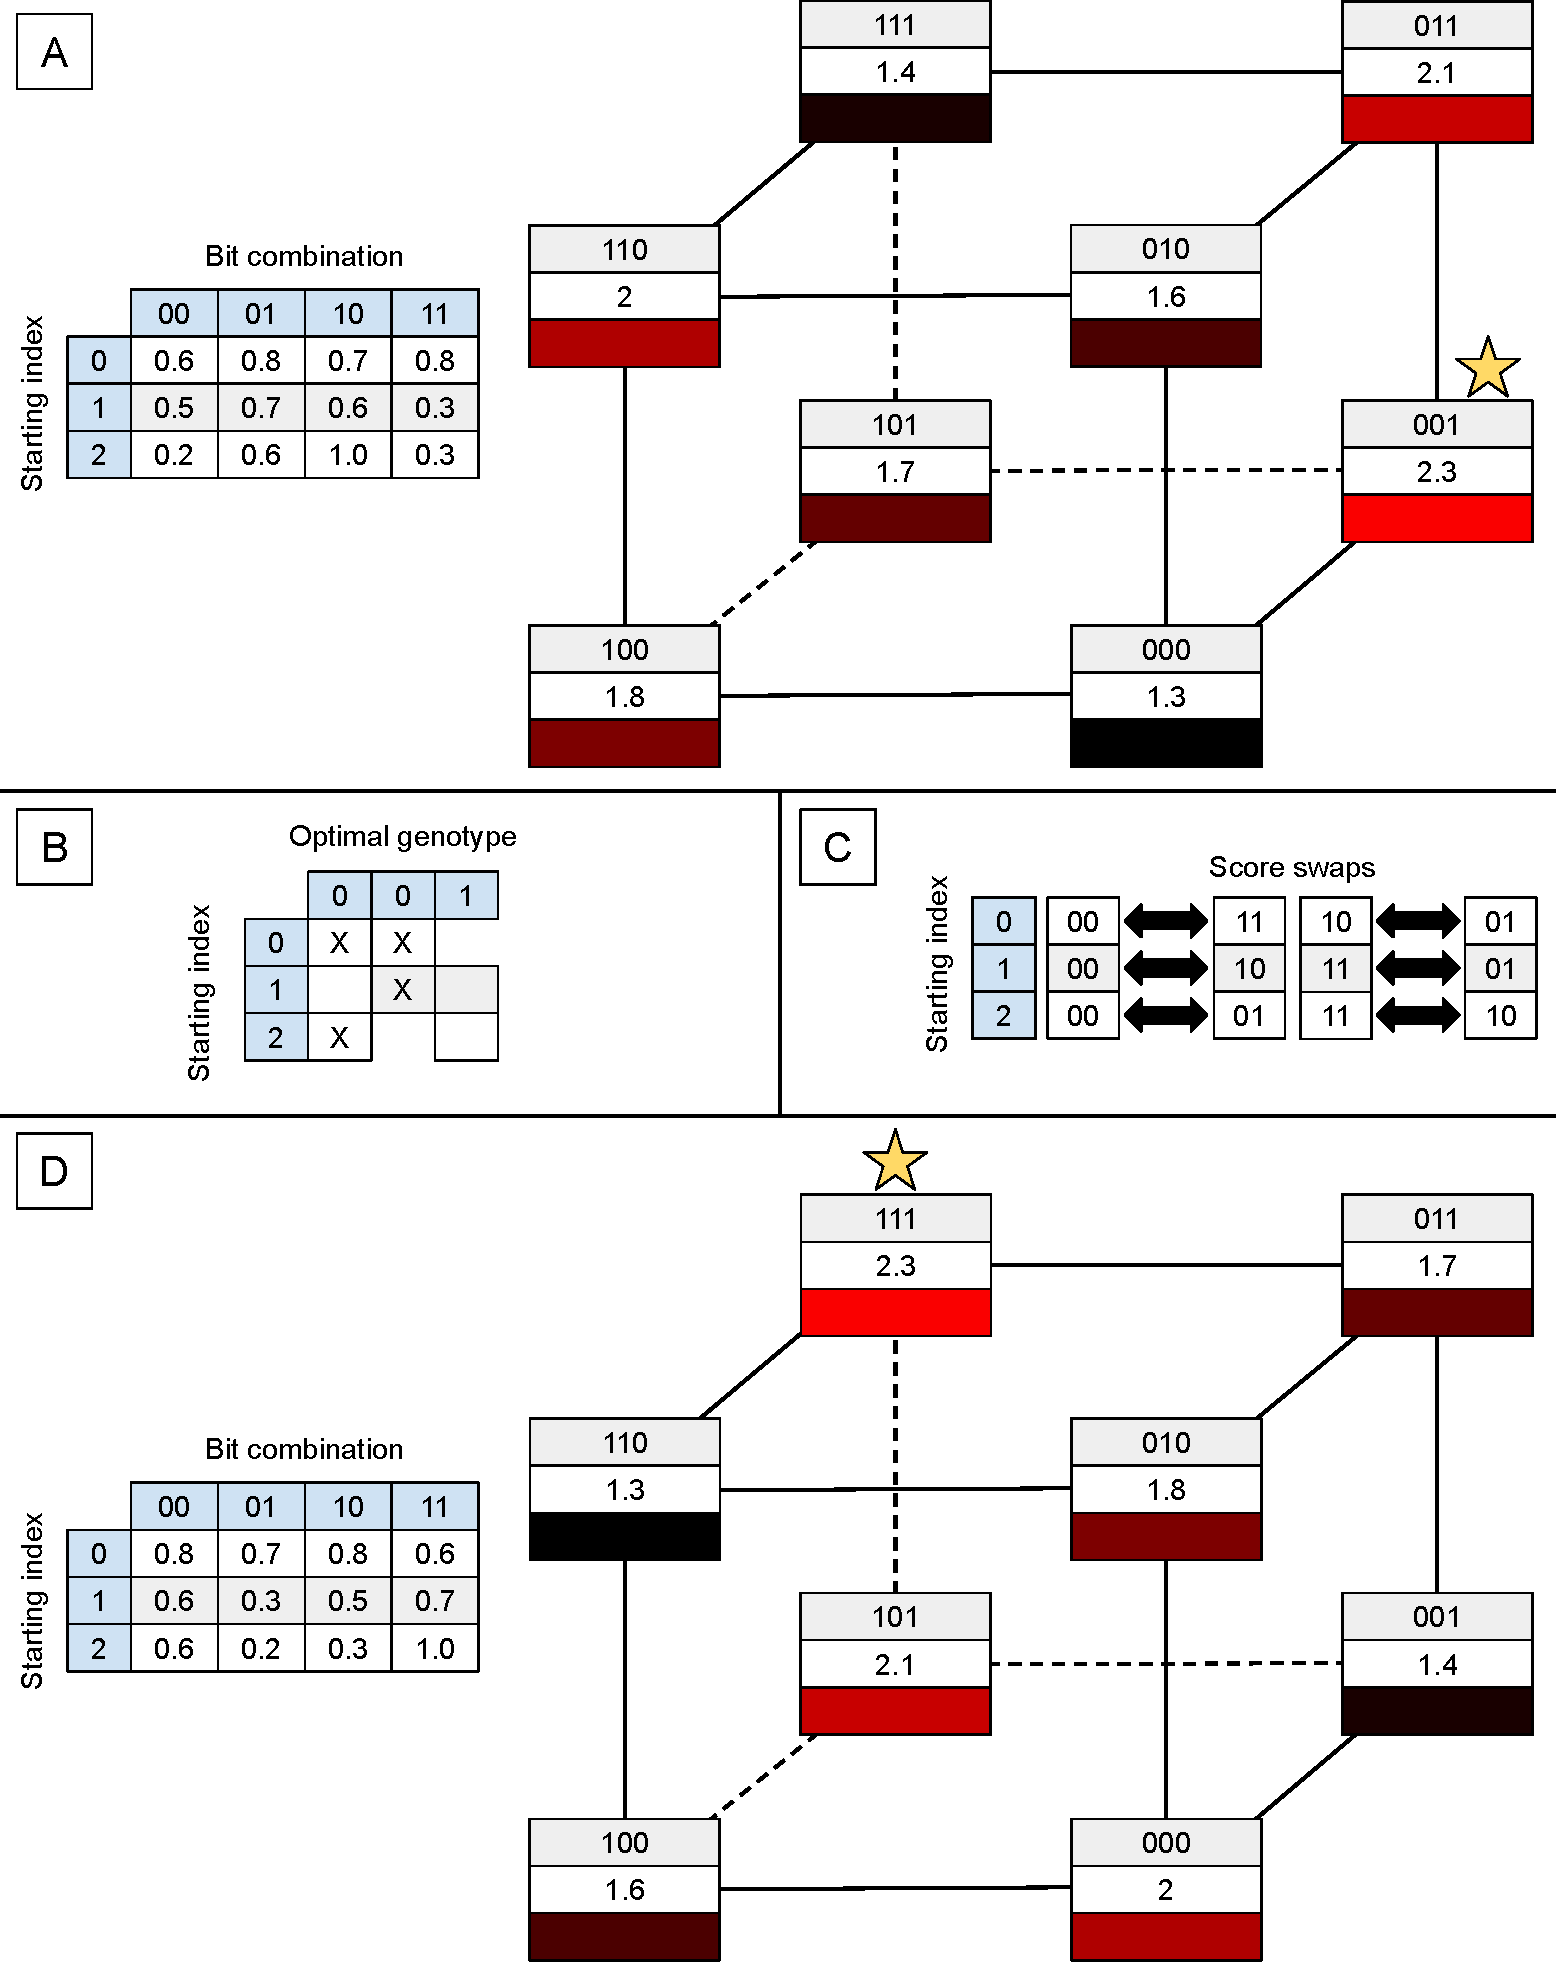
\includegraphics[width=0.9\textwidth]{04_simplified_model/media/rotating_landscape.pdf}
%     \caption{
%         An example of rotating an NK landscape where $N=3$ and $K=1$. 
%         Panel A shows the original landscape, including the score table and the visualized landscape. 
%         The yellow star shows the genotype with optimal fitness, 001. 
%         Panel B shows the mask of which bits need flipped, in this case the first two. 
%         These flips are demonstrated in Panel C.
%         At the first starting index both bits are flipped, while only one bit is flipped in the other indices. 
%         Finally, Panel D shows the resulting score table and landscape, which is isomorphic to the first but now 111 has maximal fitness.
%     }
%     \label{fig:simplified_model:rotating_landscape}
% \end{figure}

% We make one change to the NK landscape to make our analysis easier. 
% Traditionally in bitstring models, the distance between two bitstrings is calculated as their Hamming distance.
% To make comparisons with the global optimum easier, we propose to ``rotate'' the NK landscape. 
% Once the global optimum is known (in this case, found via brute force enumeration), the scoring rules of the landscape can be changed such that the global optimum occurs at the bitstring of all ones. 
% To accomplish this, for every zero in the original global optimal bitstring, we must swap the scores anywhere this bit is used. 
% This does not change the topology of the landscape, it merely re-labels the genotypes within.
% Figure \ref{fig:simplified_model:rotating_landscape} shows an example 
% Note that this is equivalent to XOR-ing a bitstring with the complement of the global optimum bitstring before evaluating its score.
% Once this transformation is complete, the distance to the optimal, successful, genotype is simply the number of zeros in a genome. 

I will conduct evolution like a traditional synchronous-generation genetic algorithm. 
I will seed the initial population of bitstrings with the genotype being tested, and evaluate each bitstring on the landscape. 
After this evaluation, I will select parents via a mix of elite selection (to ensure the optimal genotype persists if it is discovered) and tournament selection. 
Finally, all parents will be copied and possibly mutated, creating the next generation to be evaluated. 
I will then repeat this process until a stopping criterion is met. 

Quantifying the potentiation of a genotype is done by seeding some number of evolutionary replicates with that genotype and measuring the percentage of those replicates that evolve the target trait (as originally introduced in \citet{blountHistoricalContingencyEvolution2008}). %the percentage of replicates that evolve the target behavior when starting at that genotype. 
Typically, this is only measurable via multiple replay experiments that restart evolution at specific points along a lineage. 
Because I am using bitstrings, I am able to enumerate potentiation for \textit{all} possible genotypes in a landscape, creating a ``potentiation landscape''. 
This requires nontrivial effort, as there are $2^{N}$ possible genotypes in an $N$-length bitstring, and analyzing each genotype requires multiple evolutionary replicates started from it (here I use 50). 
%Once the 50 replicates for a given genotype are finished, I calculate potentiation as the percentage of those replicates evolved the target trait. 
%For the first time, we will be able to observe how potentiation changes with every step, both along a lineage and in the neighboring steps that could have been taken. 
This approach limits the size of landscapes that I can enumerate. 
As such, I propose to start by analyzing landscapes where $N \in \{10,12,14,16\}$ bits.
For each of these $N$ values, I will also vary $K \in [0, N - 1]$.
To ensure we observe the diversity landscapes can have at a particular combination of $N$ and $K$, I will enumerate the potentiation landscape for 30 landscapes at each pair of values. 

% First, we define the patterns of potentiation that we hope to observe in the system. 
% These are refined from the exploratory work of Chapter \ref{chap:replaying_associative_learning}, and are subject to change as we finish Chapters \ref{chap:replaying_associative_learning} and \ref{chap:varying_environments}.
% The three types of potentiation are: 
% \begin{enumerate}
%     \item Mutating toward the behavior, reducing the number of mutations to get there in the future
%     \item Shifting toward another genotype with the behavior that has a larger fitness advantage
%     \item Moving to another point in the genotype space such that the path toward the behavior becomes easier to traverse
% \end{enumerate}
% The three types of potentiation are visualized in Figure \ref{fig:06:conceptual_figure}

% We have constructed a bitstring model that allows for all three types of potentiation. 


% \begin{figure}
%     \centering
%     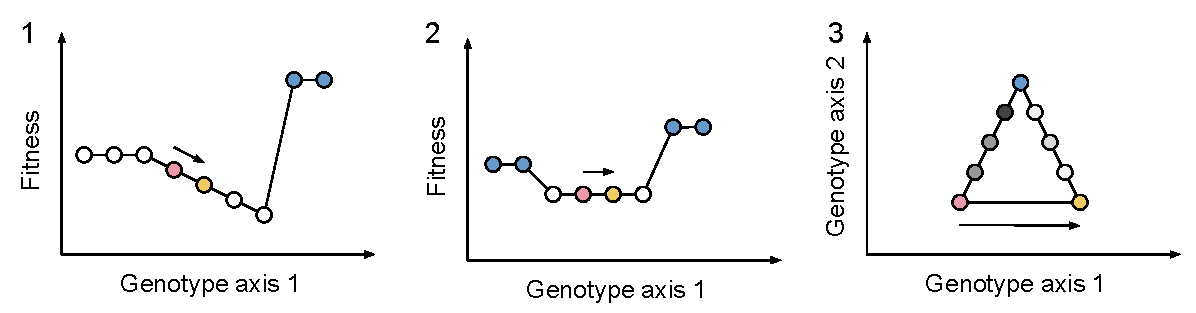
\includegraphics[width=0.9\textwidth]{04_simplified_model/media/potentiation_types_conceptual_figure.pdf}
%     \caption{
%     A conceptual figure demonstrating the three types of potentiating mutations.
%     The first two subplots show fitness on the y-axis, while the final subplot requires two genotype-space axes. 
%     All plots show the starting genotype in red, the potentiated mutant in yellow, and one or more genotypes with the focal trait in blue.
%     Arrows also show the mutation. 
%     The final subplot shows fitness of intermediate points on a grayscale axis with lighter colors being more fit.}
%     \label{fig:06:conceptual_figure}
% \end{figure}

\subsection{Proposed comparative analyses}

I plan to conduct two comparisons of potentiation: one between the NK landscape and the associative learning Avida domain, and the other across different $N$ and $K$ values within the NK landscape. 
However, the measurements taken in the associative learning domain were looking at potentiation along a lineage, not over the entire landscape (see \ref{sub:potentiation_measures} for the list of measurements). 
I will calculate the lineage metrics in the NK landscape by rerunning replicates at particular genotypes, tracking the evolving phylogenies. 
Specifically, I will target genotypes with low potentiation values, below 10\%, in order to create a fair comparison with the low initial potentiation seen in the associative learning results. 
Here, however, we do not need to perform replay replicates along these lineages, as we already know the potentiation of every possible genotype.
We merely need to map genotypes along the lineage with their potentiation values. 
Once potentiation has been assigned to every genotype along the lineage, we can calculate the potentiation measurements as normal. 

After these measurements have been collected, I will compare the distributions of each with those found in the associative learning environment of Chapter \ref{chap:replaying_associative_learning}.
As an example, I will test if there is a significant difference in the largest single-step potentiation gain between the two systems. 
Not all measurements translate to this system, but largest single-step potentiation gain/loss, the distance to the target trait from the potentiating mutations, and distributions of fitness effect apply equally to both systems. 
This will provide the first comparison of potentiation across environments and representations. 
If the distributions are similar, that would be strong evidence that there are general trends in potentiation. 
If, instead, significant differences exist, that will also provide information on what our simplified model might be missing. 

Next, I plan to perform a similar analysis across $K$ values in the NK landscape. 
Since $K$ controls the level of epistasis in the landscape, these tests will highlight the effect that epistasis has on our potentiation measurements. 
I will perform this analysis for each of the $N$ values tested. 
I will compare the relevant potentiation measurements across the set of $K$ values, seeing which ones statistically differ. 
%For example, does the fitness effect of potentiating mutations change as we increase the level of epistasis in the system? 
For example, I expect increased epistasis to make the landscapes more deceptive and thus increase the effect size of potentiating mutations.
Likewise, I will examine the consistency of the effect of $K$ on potentiation, by comparing fixed $K$ values across each $N$.

For both of these comparisons, I will conduct a Kruskal-Wallis test across all groups to see if any significant difference is found \citep{kruskal_use_1952}. 
If a difference is present, I will then conduct pairwise Mann-Whitney-Wilcoxon tests to determine which pairs of groups differ \citep{10.2307/3001968}.
Finally, I will apply Holm-Bonferroni corrections for multiple comparisons where needed \citep{holmSimpleSequentiallyRejective1979}.

% I propose a set of analyses that expand upon the work proposed in Chapter \ref{chap:replaying_associative_learning}. 
% Overall, I will enumerate multiple landscapes for various values of $N$ and $K$, calculating potentiation for every possible genotype. 
% This will allow us to compare the fitness landscape with the ``potentiation landscape'' for the first time. 
% As such, we can examine the relationships between fitness, potentiation, the distance to the target genotype, $N$, and $K$.
% Additionally, in enumerating genotype space, we will be running multiple evolutionary replicates from each genotype. 
% We can examine the dominant lineage of any of these replicates, allowing us to see how potentiation changed over time. 
% This allows us to compare potentiation in this system to that of Chapter \ref{chap:replaying_associative_learning}, which looked at the potentiation of associative learning in Avida. 

% To map the potentiation landscape, I will quantify potentiation at every possible genotype. 
% In our bitstring model, that can be accomplished by testing every bitstring in $[0, 2^{N} - 1]$.
% For a given genotype, we measure potentiation in the same way as previous work \citep{blountHistoricalContingencyEvolution2008} (Chapter \ref{chap:alife_submission}); we run a large number of evolutionary replicates starting from that genotype and calculate the percetange of those replicates that evolve the target trait. 
% This has traditionally been done along a lineage, but the same test holds for arbitrary genotypes. 
% The one difference is the time allowed in those evolutionary replicates. 
% Along a lineage, time is typically controlled such that the number of generations before that time point is subtracted from a total generation budget, ensuring that genotypes later in the lineage see fewer generations than those earlier. 
% Here we simply give all genotypes the same budget of 5,000 generations, which should be more than enough to traverse stable point. 
% I will perform these enumerations on 50 landscapes per treatment, varying $N \in [10,16]$ and $K \in [0,4]$ for a total of 35 treatments and 1750 landscapes. 
% This requires substantial computation effort, but preliminary experiments show that a 10-bit landscape can be fully enumerated in a matter of hours (a comparable amount of time to one initial replicate in Chapter \ref{chap:alife_submission}).

% Once the landscapes have been enumerated, I will analyze the relationships within and between treatments. 
% Within a treatment (a combination of $N$ and $K$), I will examine the distributions of potentiation of all genotypes.
% A Kruskal-Wallis test will determine if any significant variation exists among these distributions \citep{kruskal_use_1952}. 
% In each treatment, I will also inspect the relationship between fitness and potentiation for a sampling of landscapes. 
% I hypothesize that low potentiation can arise from populations reaching a local optima, preventing them from reaching the global optimum because valley crossing would be required. 
% If this is the case, I expect to see a negative correlation between the fitness and potentiation. 
% However, due to the nature of NK landscapes, I also expect points close to the global optimum to also have high fitness, while also having high potentiation. 
% As an illustrative example, think of all $N$ genotypes that are one step away from the global optimum; these genotypes are likely to have high fitness (though not guaranteed), however, they are guaranteed to have lower fitness than the global optimum and thus a very high potentiation. 
% As such, I expect \textit{many} genotypes to experience a negative correlation between fitness and potentiation, but with exceptions in genotypes that are close to the global optimum and have a path of ever-increasing fitness to that optimum. 
% Because the number of possible direct paths to the optimum increases factorially with distance to the global optimum, I will inspect these data with respect to their distance to the optimum. 
% I expect to see the negative correlation between fitness and potentiation to break down for short distances. 

% In calculating these potentiation values, I will be running evolutionary replays. 
% We can pull the dominant lineage of any of these replays to look at how potentiation changes throughout the lineage. 
% However, unlike previous work, we do not need to calculate the potentiation for the lineage, as we will know the potentiation for every possible genotype. 
% One important difference between this system and Avida is that these NK landscapes have no concept of a ``default ancestor''. 
% This means we do not have a single starting genotype from which we can observe how potentiation changes over different lineages. 
% Instead, we can sample successful lineages of genotypes that evolved the target trait from genotypes that have intermediate potentiation. 
% Genotypes that have 0\% or 100\% potentiation are not of interest, but all other values potentially are. 
% Specifically, I will sample lineages from genotypes with potentiation between 2\% and 15\% so they are comparable to those in Chapters \ref{chap:alife_submission} and \ref{chap:replaying_associative_learning}. 

% Once these lineages have been identified, I will collect the same potentiating measurements described in Section \ref{sub:potentiation_measures}. 
% I will then conduct statistical comparisons between the two systems. 
% As an example, I will test if there is a significant difference in the largest single-step potentiation gain between the two systems. 
% Not all measurements make sense in this system, but largest single-step potentiation gain/loss, the distance to the target trait of potentiating mutations, and distributions of fitness effect apply equally to both systems. 
% This will provide the first comparison of potentiation across environments and representations. 
% If the distributions are similar, that would be strong evidence that there are general trends in potentiation. 
% If, instead, significant differences exist, that will also provide information on what our simplified model might be missing. 

\subsection{More advanced analyses} 

Finally, there are some analyses that are tractable in the NK landscape that were infeasible in Avida.
Indeed, the power of being able to generate a potentiation landscape suddenly makes many additional analyses possible. % allows many additional analyses to suddenly become possible.
Local optima can be counted in the NK model, allowing me to investigate the relationship between potentiation and the number of local optima in the landscape. 
Similarly, the enumeration of both the fitness and potentiation landscapes will allow me to examine correlations between potentiation and fitness for individual genotypes. 
Due to local optima, I expect potentiation to decrease with fitness, but I also expect this distribution to be bimodal as genotypes close to the global optimum should have both high fitness and high potentiation. 
For any optimum, we can determine the set of genotypes that have a path to that optimum that monotonically increases in fitness (i.e., the basin of attraction for that optimum \citep{ostmanPredictingEvolutionVisualizing2014}). 
We can then see if crossing into the set of genotypes that have a path to the global optimum increases potentiation. 
However, the global optimum entering that set may not be enough; we may not see jumps in potentiation until the we reach a genotype where \textit{only} the global optimum is in that set.
%I expect that mutating to a genome that \textit{only} includes the global optimum in that set to maximize potentiation. 

In Chapter \ref{chap:alife_submission}, I inspected the two-step mutational neighborhood in an attempt to identify how potentiating mutations interacted with the target trait. 
The limited scope of that analysis brings its usefulness into question. 
In this NK landscape, however, we can exhaustive examine each genotype in its relationship to the local mutational neighborhood. 
This will allow me to investigate how often changes to the $n$-step mutational neighborhood translate to meaningful differences in potentiation. 
We can calculate the fraction of $n$-step mutants that are both beneficial and closer to the target trait. 
%This is effectively testing the level of epistasis up to $N$ steps out. 
How well does this correlate with potentiation? 
If we see that increasing this fraction for one- and two-step neighbors correlates well with potentiation, then this may be useful in more complex systems. 
If there is no strong signal, then this analysis may not be worth continuing in the future. 
%Analysis of the mutational neighborhood, as in Chapter \ref{chap:replaying_associative_learning}, also becomes much easier in the NK landscape. 
%This allows me to see how potentiating mutations effect the distance to the global optimum. 

%By leveraging search algorithms, 
I will also test if the probability of the most likely path from a given genotype to the target trait is a strong indicator of potentiation. 
By enumerating the fitness landscape, I can compare the fitness between one genotype and all $N$ of its one-step mutants. 
Assuming a mutation occurs, I can use the fitness values of each mutant to create the probability that each mutation would be selected (this varies with several factors, such as the selection scheme in use). 
By doing this for every genotype, I can create a graph of the entire genotype space with genotypes as nodes and their transition probabilities as weighted edges. 
Next, I will perform a negative log transformation on each weight. 
This will transform the probabilities into positive values, with smaller probabilities converting to larger values. 
Due to the nature of logarithms ($log(ab) = log(a) + log(b)$), summing these log-transformed values is the equivalent to multiplying the underlying probabilities. 
As such, this approach allows us to perform a search from a given genotype to the target trait using Dijkstra's algorithm. 
This analysis will return the \textit{most likely} path through genotype space to get from that genotype to the target. 
I will calculate this value for each genotype, and then analyze its relationship with potentiation. 
Since multiple adaptive paths between a genotype and the target can exist, I expect that, in many cases, this measure fails to accurately predict potentiation. 
Future work can then expand on this analysis by finding the $k$ shortest paths to the target trait, and seeing how many paths are required to accurately approximate potentiation \citep{eppsteinFindingShortestPaths1998}. 


\subsection{Broader impacts}

%This work has the potential to provide evidence for or against patterns in potentiation across systems. 
This work will be the first empirical measure of patterns in potentiation across systems.
Compared to Chapter \ref{chap:replaying_associative_learning}, if we see similar patterns in potentiation, then we can start to consider that these patterns may be generally applicable, at least in digital evolution but potentially into natural systems. 
If not, we can dive into the differences in patterns to begin asking if other systems will be more like one system or the other. 
Additionally, this work will provide insight into how we measure potentiation and characterize potentiating mutations, and these landscapes will provide a second data set for future comparative studies. 

% Talk about how we can explore our intuition and approximations of potentiation in this system?

If I find evidence of interesting potentiation dynamics in this system, that will help establish NK landscapes as a useful tool for investigating potentiation. 
An NK landscape where $K = 0$ is just a single hill to climb, and as such I expect all genotypes in that landscape to have 100\% potentiation. 
If I see potentiation vary more across landscapes as $K$ increases, that will provide support for the hypothesis that epistatic interactions are key to potentiation. 
They might not be the only factor though, and future models may need to expand beyond the traditional NK model. 
If, for instance, I do not see large jumps in potentiation, I may need stronger binary ``on/off'' forms of potentiation. 
A simple example would be a bitstring environment where the first half of the bitstring is evaluated on one NK landscape and the second half on another, with the target trait being optimal genotypes in both landscapes. 
If I limit fitness such that the second half of the bitstring only contributes to fitness if the first half is at the global maximum, then I would expect to see a drastic increase in potentiation when the first half reaches that optimal genotype. 
This model would more directly simulate required building blocks in the evolution of the target trait. 
There are many ways that we could extend the traditional NK model, and this work will help shape those future studies, if needed. 

\section{Preliminary results}

To ensure that potentiation in NK landscapes is not entirely trivial, I ran some very early preliminary data. 
I selected $N=10$ and enumerated potentiation in 50 landscapes each of $K \in \{0,1,2,3\}$.
For each landscape, I ran 50 replicates from every genotype (1,024 genotypes per landscape) to quantify potentiation at that point. 
%These data are not fully analyzed and these plots are rough, this was last-minute data to make sure this environment was worth looking into. 

\begin{figure}[h!]
    \centering
    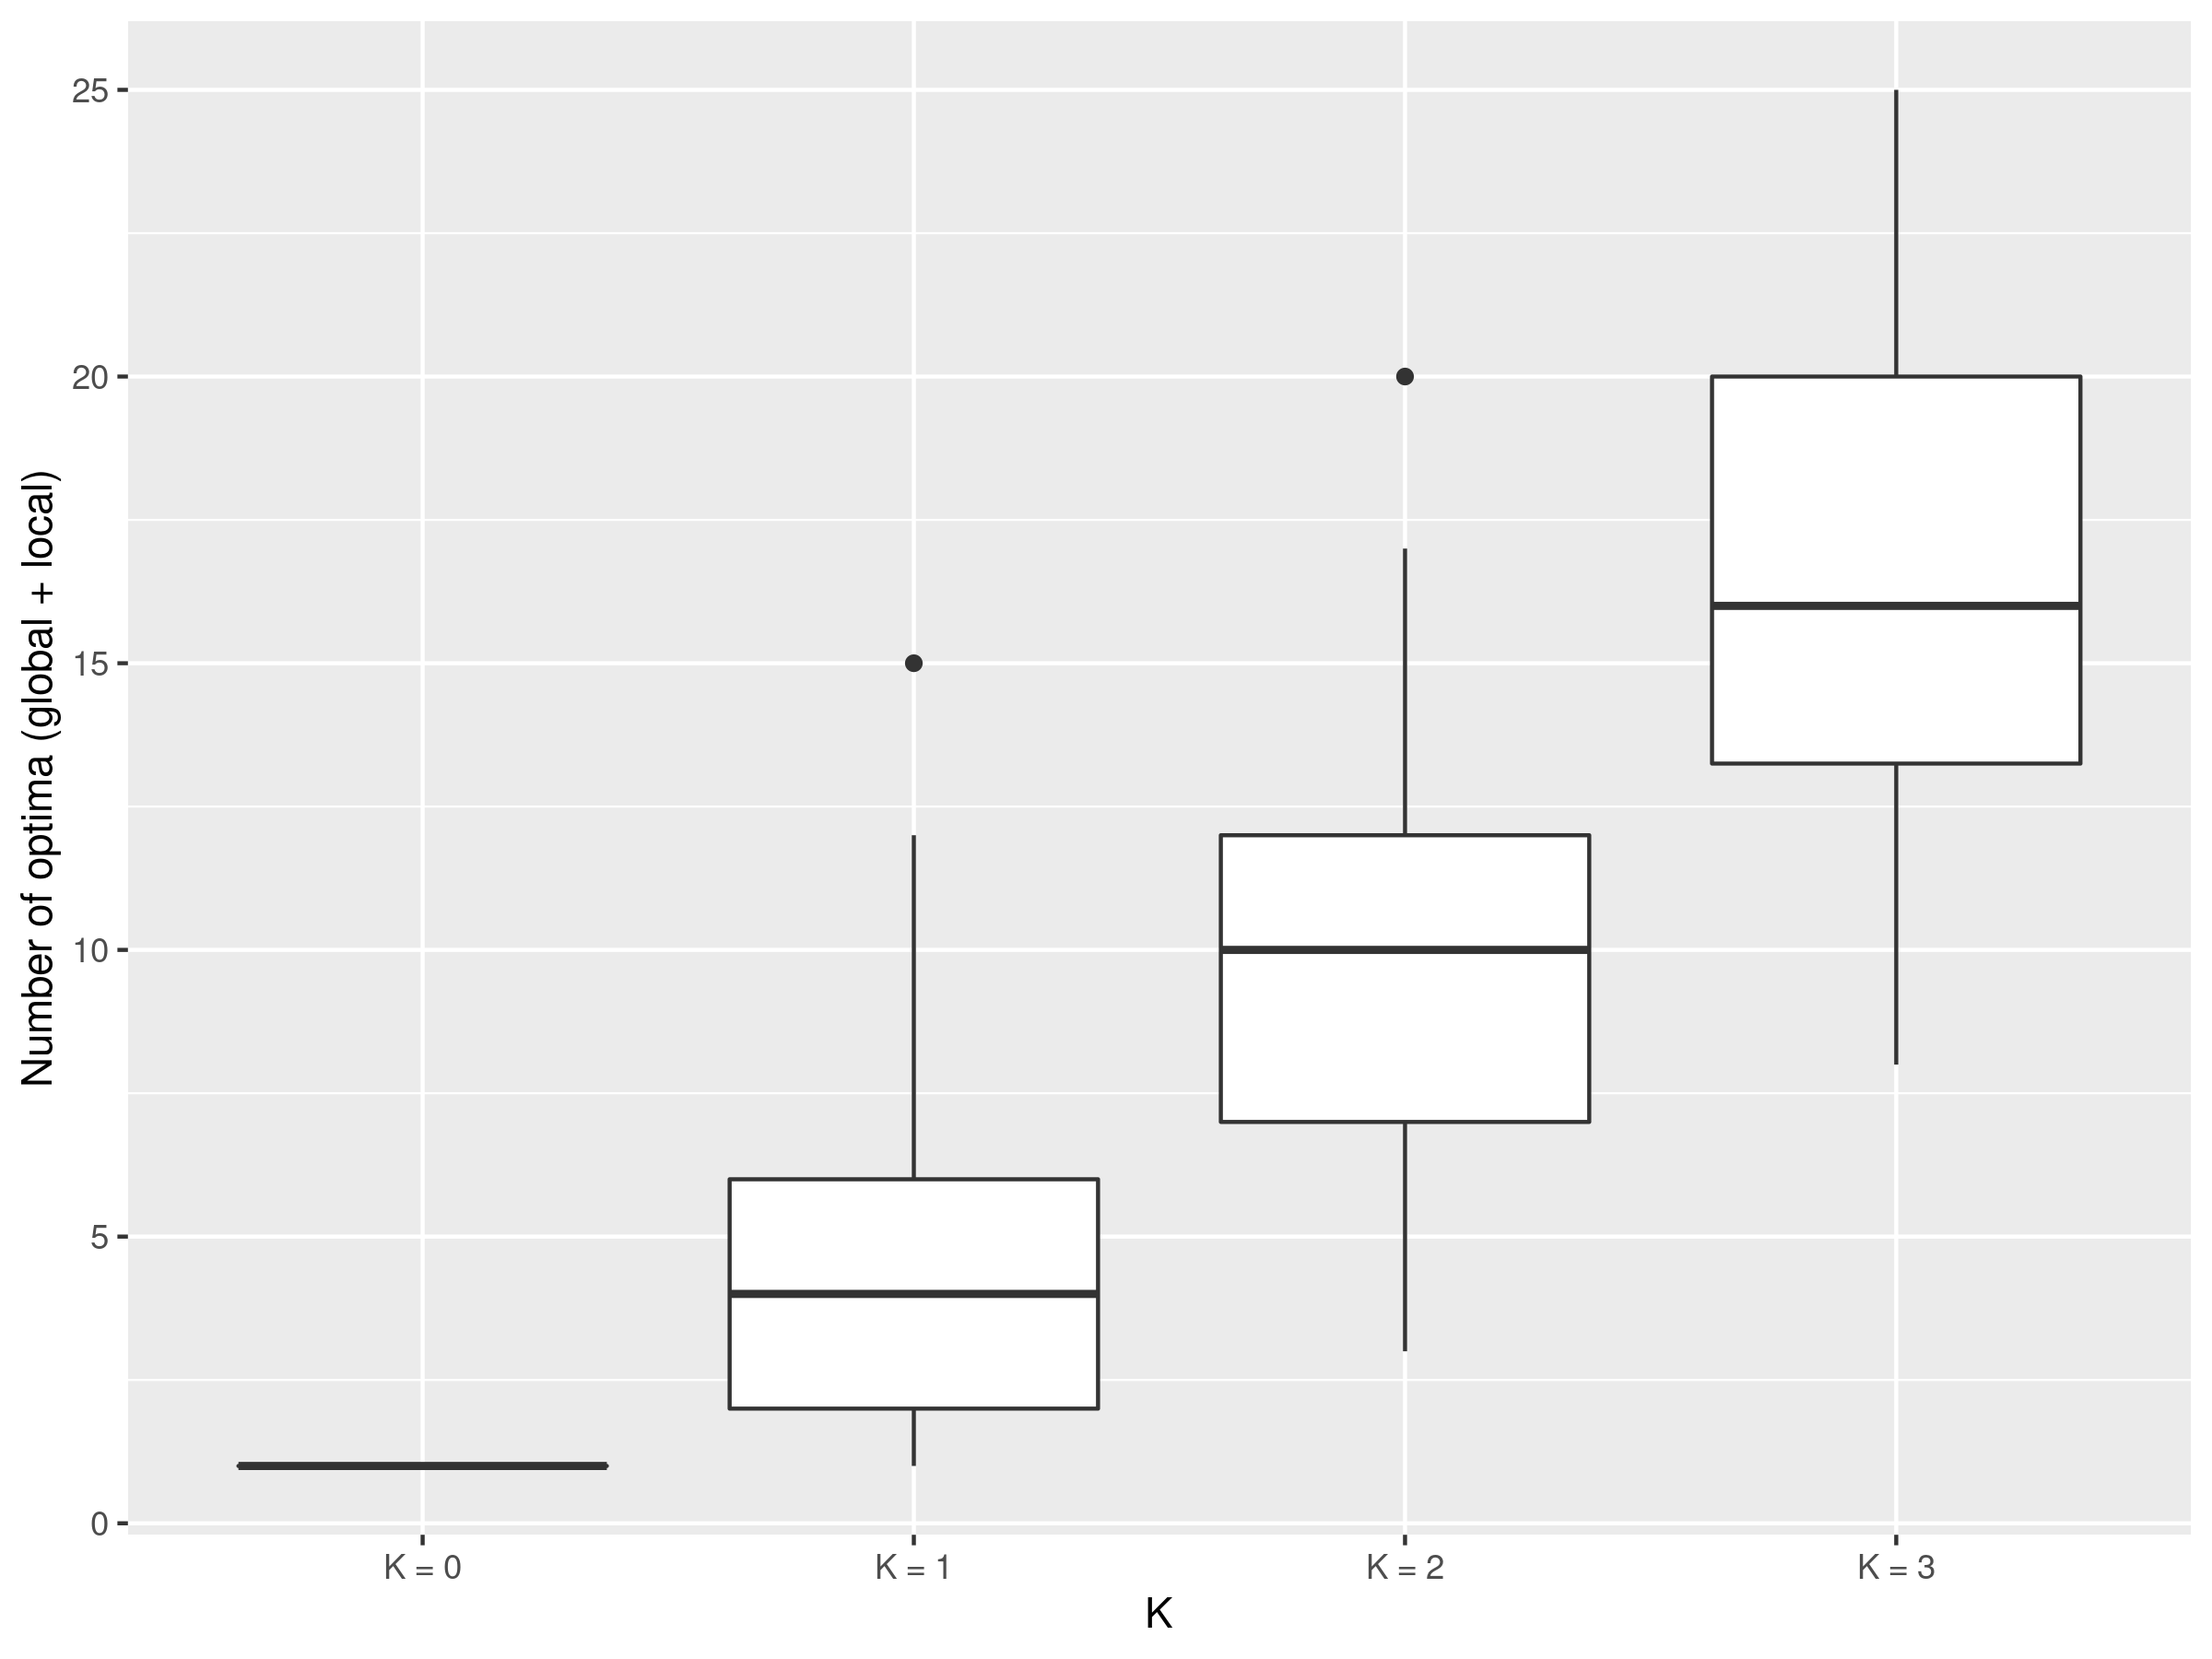
\includegraphics[width=0.95\textwidth]{04_simplified_model/media/num_peaks.png}
    \caption{
        Boxplots showing the number of peaks in all 50 landscapes of a given $K$ value. 
    }
    \label{fig:simplified_model:num_peaks}
\end{figure}

First, Figure \ref{fig:simplified_model:num_peaks} shows the number of peaks at each $K$ value. 
Here we define a peak as a genotype that has higher fitness than the $N$ genotypes around it; this definition includes local optima as well as the global optimum \citep{ostmanPredictingEvolutionVisualizing2014}. 
NK landscapes are often described as ``tunably rugged'', with larger $K$ values creating more rugged landscapes due to increased epistatic interactions. 
We see exactly that here, as the number of peaks increases smoothly as we increase $K$. 

\begin{figure}[h!]
    \centering
    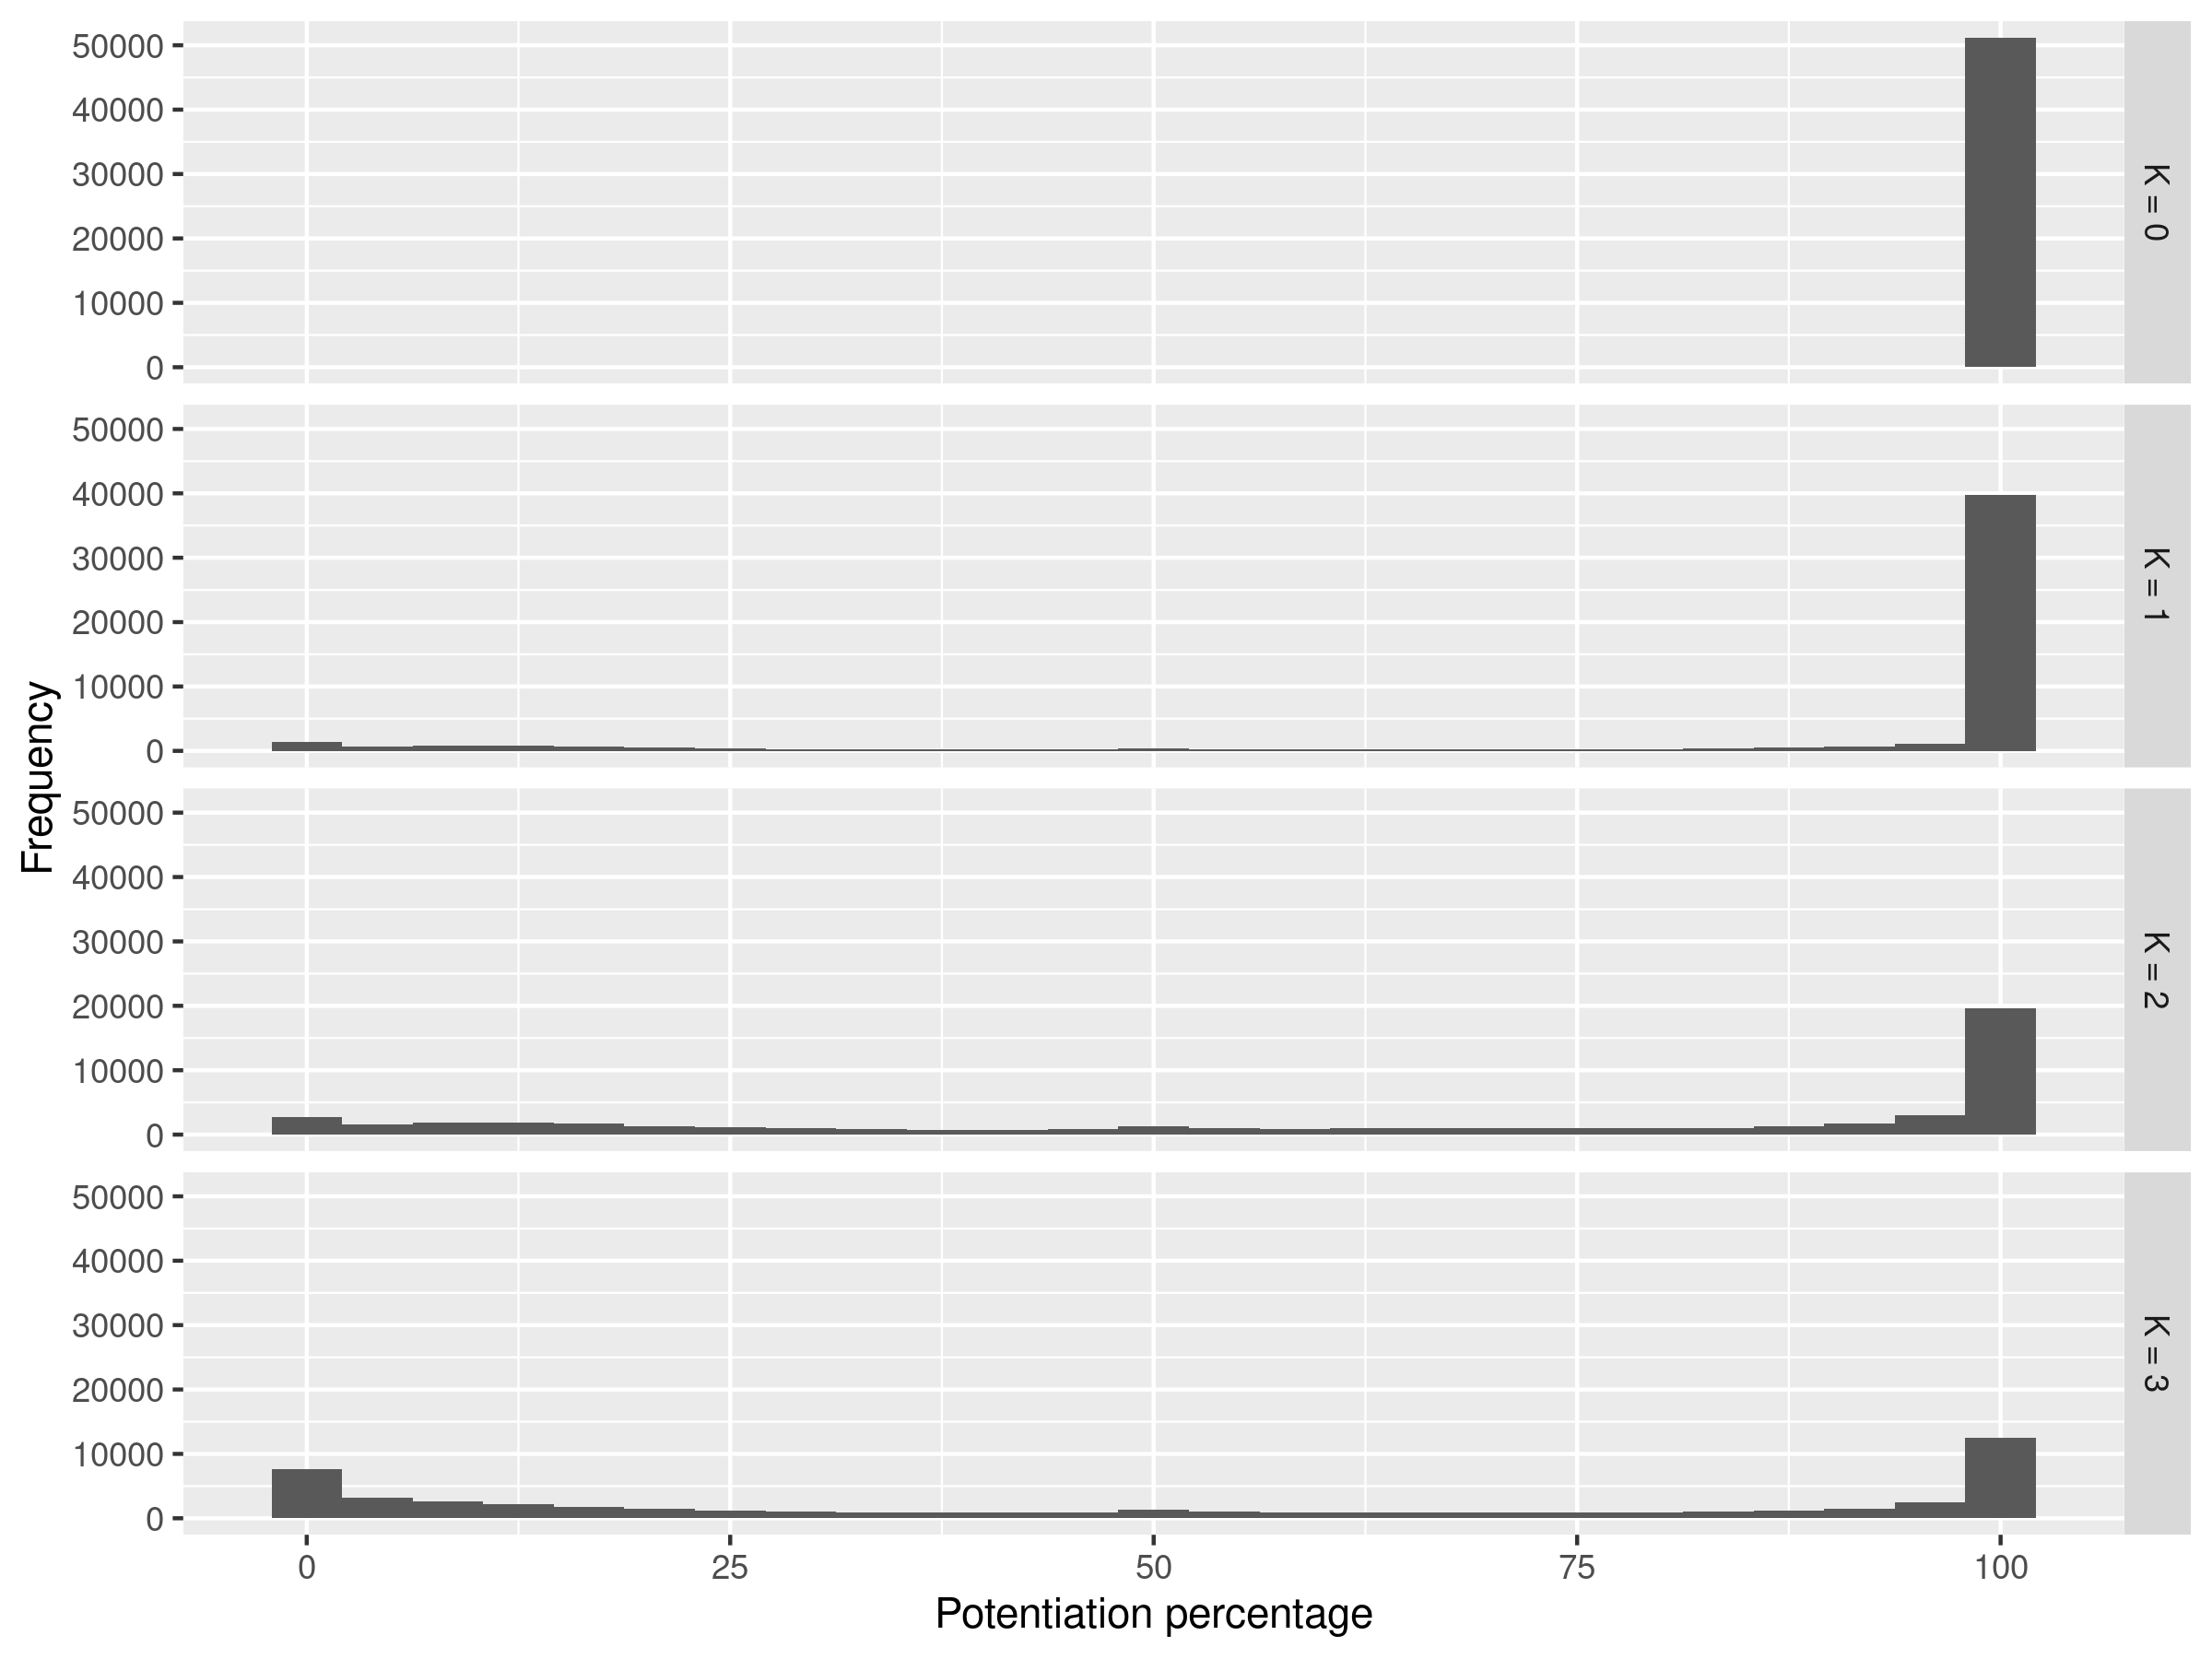
\includegraphics[width=0.95\textwidth]{04_simplified_model/media/success_histogram.png}
    \caption{
        Histograms of potentiation, with one row per $K$ value.
        Each histogram includes the potentiation of all 1,024 genotypes in all 50 landscapes for that $K$ value.
    }
    \label{fig:simplified_model:potentaition_histogram}
\end{figure}

Figure \ref{fig:simplified_model:potentaition_histogram} shows the overall distribution of potentiation across all genotypes in all landscapes at each $K$ value. 
First, $K=0$ shows 100\% potentiation for every genotype in every landscape, which matches expectations as individual bits can be optimized independently (i.e., there is zero epistasis) and thus the landscape is a single hill to climb. 
As $K$ increases, we see some mass of the distribution shift from 100\% potentiation to the lower values, especially the very low values around 0\%. 
This also meets my expectation, as we have shown that increasing $K$ increases the number of local optima and thus creates more opportunities for populations to become ``stuck'' and unable to reach the global optimum. 
When it comes time to compare potentiation in this model to that in Avida, we do see genotypes with potentiation levels similar to those found in Avida, indicating that we can conduct those comparisons fairly. 

\begin{figure}[h!]
    \centering
    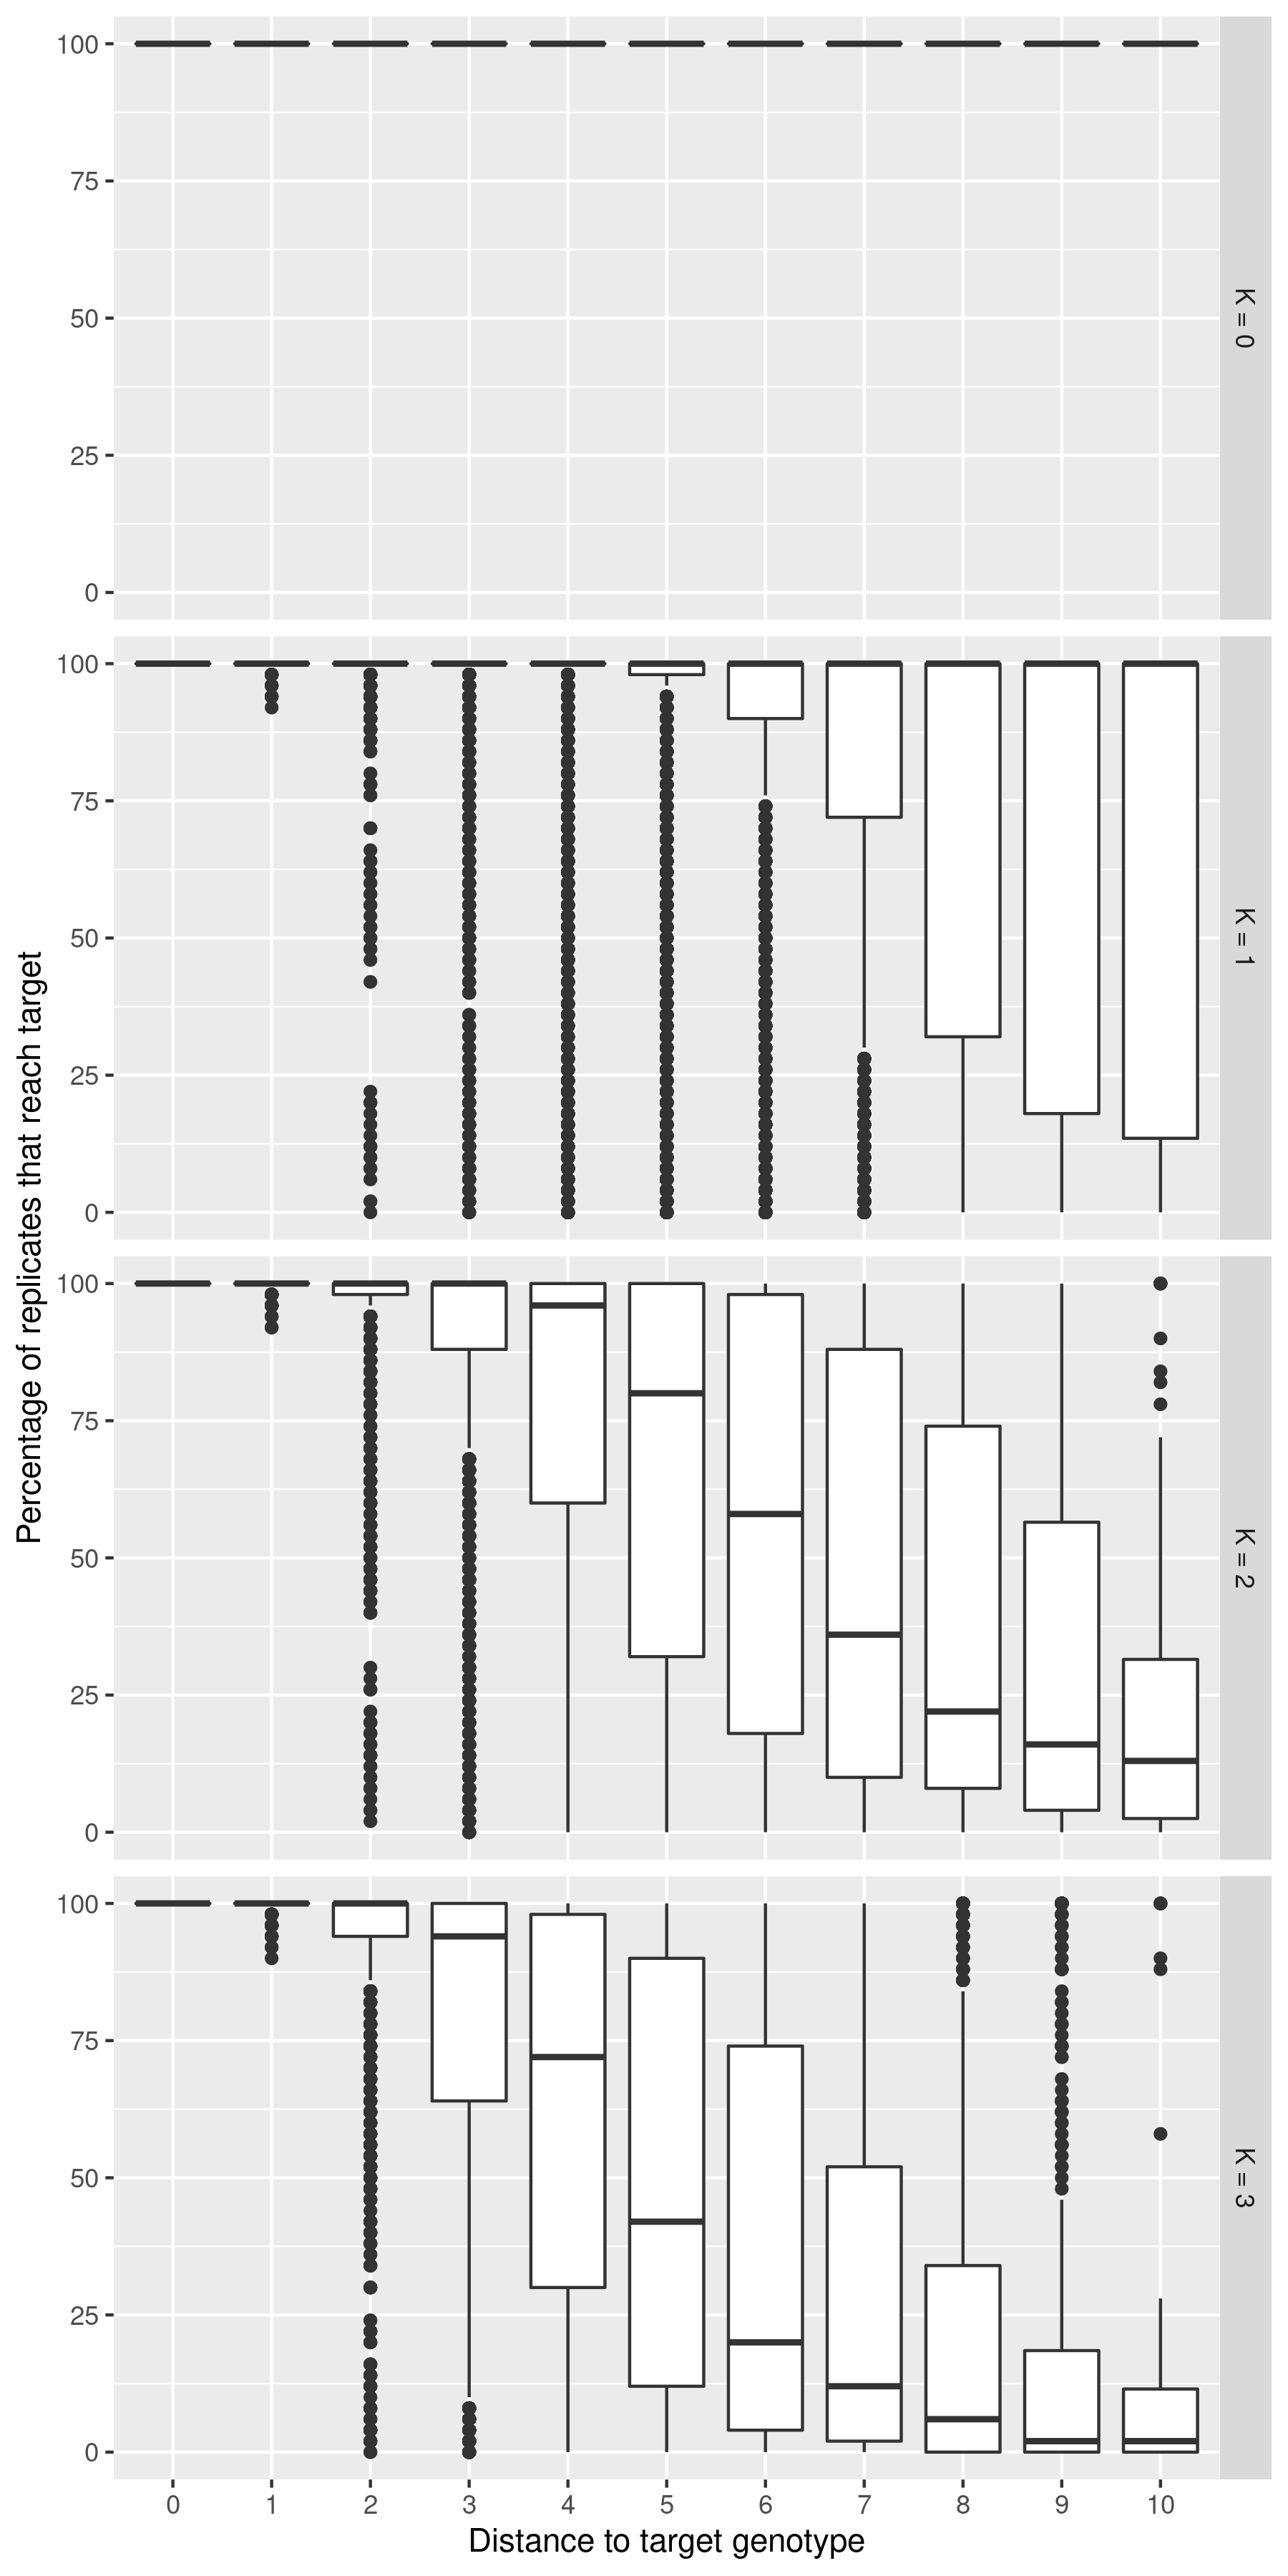
\includegraphics[width=0.6\textwidth]{04_simplified_model/media/potentiation_by_distance_boxplots.png}
    \caption{
        Boxplots showing the potentiation of genotypes at a given distance away from the global optimum. 
        Rows show the various $K$ values, and each boxplot shows all genotypes at that distance for all 50 landscapes for that $K$ value. 
    }
    \label{fig:simplified_model:distance_boxplots}
\end{figure}

Finally, Figure \ref{fig:simplified_model:distance_boxplots} shows how potentiation changes as we vary $K$ and look at the distance from a genotype to the target trait.
As we have already seen, $K = 0$ is a single hill and thus all genotypes are fully potentiated. 
Starting at $K=1$, we see that while the median potentiation stays consistently high, the lowest quartile decreases as distance from the target increases. 
At $K=2$, we see the whole distribution of potentiation shift to lower values as distance increases, with very few points at the maximum distance having high potentiation. 
This trend continues into $K = 3$, becoming more pronounced. 
Overall, Figure \ref{fig:simplified_model:distance_boxplots} meets my expectations. 
In the simpler landscapes, most genotypes have high potentiation, but as the landscapes become more rugged we see potentiation fall faster as we increase the distance to the target. 

While these data are only a shallow glance into potentiation in NK landscapes, they provide reassurance that the system is worthy of examination. % looking into.
When performing the work in earnest, I will be analyzing landscapes with higher values of $N$ and $K$. %, and performing deeper analyses by looking at aspects such as the basins of attraction to the target.
Additionally, I will be looking at the lineages of semi-potentiated genotypes, allowing me to compare the potentiation measures that will be recorded in Chapter \ref{chap:replaying_associative_learning}. 
This brief glimpse reveals promise in the system; hopefully this promise holds true and NK landscapes can help us delve further into potentiation. 